\documentclass{article}
\usepackage{amsmath}
\usepackage[mathletters]{ucs}
\usepackage[utf8x]{inputenc}
\usepackage[margin=1.5in]{geometry}
\usepackage{enumerate}
\newtheorem{theorem}{Theorem}
\usepackage[dvipsnames]{xcolor}
\usepackage{pgfplots}
\setlength{\parindent}{0cm}
\usepackage{graphics}
\usepackage{graphicx} % Required for including images
\usepackage{subcaption}
\usepackage{bigintcalc}
\usepackage{pythonhighlight} %for pythonkode \begin{python}   \end{python}
\usepackage{appendix}
\usepackage{arydshln}
\usepackage{physics}
\usepackage{tikz-cd}
\usepackage{booktabs} 
\usepackage{adjustbox}
\usepackage{mdframed}
\usepackage{relsize}
\usepackage{physics}
\usepackage[thinc]{esdiff}
\usepackage{fixltx2e}
\usepackage{esint}  %for lukket-linje-integral
\usepackage{xfrac} %for sfrac
\usepackage[colorlinks=true]{hyperref} %for linker, må ha med hypersetup
\usepackage[noabbrev, nameinlink]{cleveref} % to be loaded after hyperref
\usepackage{amssymb} %\mathbb{R} for reelle tall, \mathcal{B} for "matte"-font
\usepackage{listings} %for kode/lstlisting
\usepackage{verbatim}
\usepackage{graphicx,wrapfig,lipsum,caption} %for wrapping av bilder
\usepackage{mathtools} %for \abs{x}
\usepackage[norsk]{babel}
\definecolor{codegreen}{rgb}{0,0.6,0}
\definecolor{codegray}{rgb}{0.5,0.5,0.5}
\definecolor{codepurple}{rgb}{0.58,0,0.82}
\definecolor{backcolour}{rgb}{0.95,0.95,0.92}
\lstdefinestyle{mystyle}{
    backgroundcolor=\color{backcolour},   
    commentstyle=\color{codegreen},
    keywordstyle=\color{magenta},
    numberstyle=\tiny\color{codegray},
    stringstyle=\color{codepurple},
    basicstyle=\ttfamily\footnotesize,
    breakatwhitespace=false,         
    breaklines=true,                 
    captionpos=b,                    
    keepspaces=true,                 
    numbers=left,                    
    numbersep=5pt,                  
    showspaces=false,                
    showstringspaces=false,
    showtabs=false,                  
    tabsize=2
}

\lstset{style=mystyle}
\author{Oskar Idland}
\title{Oblig 5}
\date{}
\begin{document}
\maketitle
\newpage

\subsection*{Problem 5.6 (H)}
\subsection*{a)}
The possible values we can measure, are the eigenvalues of the $\hat{L}_z$ operator. These are given by $ℏm \ ,\ m ∈ [-l, l]⋃ℤ$ We can calculate the probability of measuring a given eigenvalue $ℏm$ by calculating the projection of the state vector onto the eigenstate of $ℏm$. As the state vector is given by a basis of the angular momentum eigenkets, their orthonormality dictates that $l = 1$ and $m ∈ [0, 1]$:
\[
P(0) = \left|\bra{1,0}\ket{ψ}\right|^2 = \left|a_0\right|^2 
\]
\[
P(ℏ) = \left|\bra{1,1}\ket{ψ}\right|^2 = \left|a_1\right|^2
\] 

\subsection*{b)}
As latitude coordinates begin from the equator, but spherical coordinates begin from the north pole, we must integrate from 0 to $π / 3$ instead of to $π / 6$. We replace the eigenkets with their corresponding spherical harmonics. 
\[
Y_{ℓ}^{m} (θ, ϕ) ∼ e^{i m ϕ} 
\]
\[
Y_{1}^{0} = \sqrt{\frac{3}{4π}}\cos θ \quad , \quad Y_{1}^{1} = -\sqrt{\frac{3}{8π}}\sin θ e^{i ϕ}
\]
When using spherical coordinates we must add the Jacobian determinant to the integral.
\[
∫_{0}^{1} ∫_{0}^{2π} ∫_{0}^{π / 3} (r^2 \sin θ)\left|-a_1 \sqrt{\frac{3}{8π}}\sin θ + a_0 \sqrt{\frac{3}{4π}}\cos θ\right|^2 \ \mathrm{d}θ \ \mathrm{d}ϕ \ \mathrm{d}r
\]
\[
2π \frac{3}{8π} ∫_{0}^{π / 3} \sin θ\left(\left|a_1\right|^2 \sin^2θ +  2\left|a_0\right|^2 \cos^2 θ\right)   \ \mathrm{d}θ
\]
\[
\frac{3}{4} \left(\frac{14a_0^2 + 5a_1^2}{24}\right) = \underline{\underline{\frac{7}{16} \left|a_0\right|^2 + \frac{5}{32} \left|a_1\right|^2}} 
\]

\subsection*{c)}
The lowering and raising operator working on a state. In our case, $l = 1$ which means we can rewrite the following:
\[
L_+ \ket{l,m} = ℏ\sqrt{l(l+1) - m(m+1)} \ket{l,m+1}
\]
\[
L_- \ket{l,m} = ℏ\sqrt{l(l+1) - m(m-1)} \ket{l,m-1}
\]
as:
\[
L_+ \ket{l,m} = ℏ\sqrt{2 - m(m+1)} \ket{l,m+1}
\]
\[
L_- \ket{l,m} = ℏ\sqrt{2 - m(m-1)} \ket{l,m-1}
\]

Lets first look at a general state in the $x$-basis:
\[
\ket{1,m}_{x} = α\ket{1,-1}_{z} + β\ket{1,0}_{z} + γ\ket{1,1}_{z}
\]
We can apply the $\hat{L}_x$ operator to this state:
\[
\hat{L}_x \ket{1,m}_{x} = \frac{1}{2} \left(\hat{L}_+ + \hat{L}_-\right)\ket{1,m}_{x}
\]

For simplicity, we calculate how the lowering and raising operator works on all our kets. 
\[
\hat{L}_+ \ket{1,-1} = ℏ \sqrt{2 - (-1)(-1+1)} \ket{1,0} = ℏ\sqrt{2} \ket{1,0}
\]
\[
\hat{L}_- \ket{1,-1} = ℏ \sqrt{2 - (-1)(-1-1)} \ket{1,-2} = 0
\]
\[
\hat{L}_+ \ket{1,0} = ℏ \sqrt{2 - (0)(0+1)} \ket{1,1} = ℏ\sqrt{2} \ket{1,1}
\]
\[
\hat{L}_- \ket{1,0} = ℏ \sqrt{2 - (0)(0-1)} \ket{1,-1} = ℏ\sqrt{2} \ket{1,-1}
\]
\[
\hat{L}_+ \ket{1,1} = ℏ \sqrt{2 - (1)(1+1)} \ket{1,2} = 0
\]
\[
\hat{L}_- \ket{1,1} = ℏ \sqrt{2 - (1)(1-1)} \ket{1,0} = ℏ\sqrt{2} \ket{1,0}
\]
We can now calculate the action of the $\hat{L}_x$ operator on our general state:
\[
\hat{L}_x \ket{1,m}_{x} = \frac{1}{2} \left(\hat{L}_+ + \hat{L}_-\right)\ket{1,m}_{x} = \frac{1}{2} \left(\hat{L}_+ + \hat{L}_-\right) \left(α\ket{1,-1}_{z} + β\ket{1,0}_{z} + γ\ket{1,1}_{z}\right)
\]
\[
\hat{L}_x \ket{1,m}_{x} =\frac{1}{2} \left( ℏ\sqrt{2}α \ket{1,0}_{z} + ℏ\sqrt{2}β \ket{1,1} + ℏ\sqrt{2}β \ket{1,-1}_{z} + ℏ\sqrt{2}γ \ket{1,0}_{z} \right)
\]
\[
\underline{\hat{L}_x \ket{1,m}_{x} = \frac{ℏ\sqrt{2}}{2} \left( (α + γ) \ket{1,0}_{z} + β \left( \ket{1,1}_{z} + \ket{1,-1}_{z} \right) \right)}
\]
We also know that the operator must satisfy the following:

\[
\hat{L}_{x} \ket{1,m}_x = ℏm \ket{1,m}_{x} = ℏm \left( α\ket{1,-1}_{z} + β\ket{1,0}_{z} + γ\ket{1,1}_{z}\right)
\]
We then plug in known values of $m$ and its respective eigenket. We begin with $m = -1$.
\[
\hat{L}_{x} \ket{1,-1}_x = \frac{ℏ\sqrt{2}}{2} \left( (α + γ) \ket{1,0}_{z} + β \left( \ket{1,1}_{z} + \ket{1,-1}_{z} \right) \right) = ℏ(-1) \left( α\ket{1,-1}_{z} + β\ket{1,0}_{z} + γ\ket{1,1}_{z}\right)
\]
This gives:
\[
γ = -\frac{\sqrt{2}}{2} β 
\]
\[
α = -\frac{\sqrt{2}}{2} β = γ
\]
\[
β = -\frac{\sqrt{2}}{2} \left(α + γ\right) = -\sqrt{2} α
\]
Setting $α = 1$ and normalizing we get we get:
\[
\underline{\underline{\ket{1,-1}_x = \frac{1}{2} \ket{1,-1}_z - \frac{1}{\sqrt{2}} \ket{1,0}_z + \frac{1}{2} \ket{1,1}_z}}
\]


We now look at $m = 0$:
\[
\hat{L}_x \ket{1,0} =  \frac{ℏ\sqrt{2}}{2} \left( (α + γ) \ket{1,-1}_{z} + β \left( \ket{1,0}_{z} + \ket{1,1}_{z} \right) \right) = 0
\]
This gives:
\[
γ = -α
\]
\[
β = 0
\]
\[
α = -γ
\]
Setting $α = 1$ and normalizing we get we get:
\[
\underline{\underline{\ket{1,0}_x = \frac{1}{\sqrt{2}} \ket{1,1}_z - \frac{1}{\sqrt{2}} \ket{1,-1}_z}}
\]


We now look at $m=1$
\[
\hat{L}_x \ket{1,1} = \frac{ℏ\sqrt{2}}{2} \left( (α + γ) \ket{1,0}_{z} + β \left( \ket{1,1}_{z} + \ket{1,-1}_{z} \right) \right) = ℏ\left( α\ket{1,-1}_{z} + β\ket{1,0}_{z} + γ\ket{1,1}_{z}\right)
\]
We see this gives the same relationships, but with the opposite sign.
\[
γ = \frac{\sqrt{2}}{2} β
\]
\[
α = \frac{\sqrt{2}}{2} β = γ
\]
\[
β = \frac{\sqrt{2}}{2} \left(α + γ\right) = \sqrt{2} α
\]
Setting $α = 1$ and normalizing we get we get:
\[
\underline{\underline{\ket{1,1}_x = \frac{1}{2} \ket{1,-1}_z + \frac{1}{\sqrt{2}} \ket{1,0}_z + \frac{1}{2} \ket{1,1}_z}}
\]

Next we calculate the probability by taking the projection of $ψ$ onto the eigenkets:
\[
P(\ket{1,-1}_x) = \left|\bra{1,-1}_x\ket{ψ}_z\right|^2
\]
\[
P(\ket{1,-1}_x) = \left| \left(\frac{1}{2} \bra{1,-1} - \frac{1}{\sqrt{2}} \bra{1,0} + \frac{1}{2} \bra{1,1}\right) \left( a_1 \ket{1,1} + a_0 \ket{1,0}\right) \right|^2
\]
\[
\underline{\underline{P(\ket{1,-1}_x) = \left| \frac{1}{2} a_1 - \frac{1}{\sqrt{2}} a_0\right|^2}}
\]

\[
P(\ket{1,0}_x) = \left|\left(\frac{1}{\sqrt{2}} \ket{1,1} - \frac{1}{\sqrt{2}}\ket{1,-1} \right) \left(a_1 \ket{1,1} + a_0 \ket{1,0}\right)\right|^2  
\]
\[
\underline{\underline{P(\ket{1,0}_x) = \frac{1}{2}\left| a_1\right|^2}}
\]
\[
P(\ket{1,1}_x) = \left|\left(\frac{1}{2} \ket{1,-1} + \frac{1}{\sqrt{2}} \ket{1,0} + \frac{1}{2} \ket{1,1}\right) \left(a_1 \ket{1,1} + a_0 \ket{1,0}\right)\right|^2
\]
\[
\underline{\underline{P(\ket{1,1}) = \left| \frac{1}{2}a_1 + \frac{1}{\sqrt{2}}a_0 \right|^2}}
\]

\section*{Problem 5.7 (H)}
\subsection*{a)}
The potential energy of a Tritium atom is the same as that for the Hydrogen. 
\[
E^{H}_{n} = -\frac{1}{n^2} \frac{m}{2ℏ^2} \left(\frac{e^2}{4πϵ_0}\right)^2 = \frac{E_1}{n^2}
\]

After decay, the charge inside the atom is doubled from $e$ to $2e$. This means the potential energy is quadrupled. 
\[
E_n^{He} = - \frac{1}{n^2} \frac{m}{2ℏ^2} \left(\frac{2e}{4πϵ_0}\right)^2 = 4 \frac{E_1}{n^2}
\]

\subsection*{b)}
We know the wave function of an electron in the ground state of a hydrogen atom is given by:
\[
ψ_{100} = \frac{1}{\sqrt{π a_0^3}} e^{-r / a_0}
\]
where $r$ is the radial distance, and $a_0$ is the Bohr radius. This radius is determined by the potential energy. We need to compute a new value for this radius $a_0'$, as the potential energy has changed. We know the Bohr radius is given by: 
\[
a_0 = \frac{4πϵ_0 ℏ^2}{m e^2}
\]
The only change is that the charge $e^2$ is replaced by $2e^2$. This gives:
\[
a_0' = \frac{4πϵ_0 ℏ^2}{m 2e^2} = \frac{a_0}{2}
\]
We get a new wave function:
\[
ψ_{100}' = \frac{1}{\sqrt{π a_0'^3}} e^{-r / a_0'} = \frac{1}{\sqrt{π \left(\frac{a_0}{2}\right)^3}} e^{-r / \left(\frac{a_0}{2}\right)} = \frac{2\sqrt{2}}{\sqrt{π a_0^3}} e^{-2r / a_0}
\]
Now we can calculate the probability of finding the electron in the ground state of the Helium atom:
\[
P(\text{Ground state}) = \left|∫ ψ'^{*} ψ' \ \mathrm{d}r^3\right|^2
\]
\[
P(\text{Ground state}) =  16π^2 \frac{8}{π^2a_0^6} \left|∫_{0}^{∞} r^2 e^{-3r / a} \ \mathrm{d}r\right|^2
\]
Using integration by parts we get 
\[
P(\text{Ground state}) =  \frac{16 ⋅ 8}{a^{6}} \left| \frac{2a^3}{-27} \right|^2 ≈ \underline{\underline{0.702}}
\]

\section*{5.8 (X)}
\subsection*{a)}
The particle is in a spherically symmetrical potential, which means the potential energy is independent of the angle. This is the case as our electron is in the ground state. 

\subsection*{b)}
As we are in the ground state, the energy is not affected by the quantum number $m$. As the energy correction is proportional to $m^2$, it's only the absolute value of $m$ that matters. We know $L_z = ℏm$ which makes $H' = gFm^2$. This creates the following plot of the field $F$ and the energy $E$
\begin{figure}[h!]
\centering
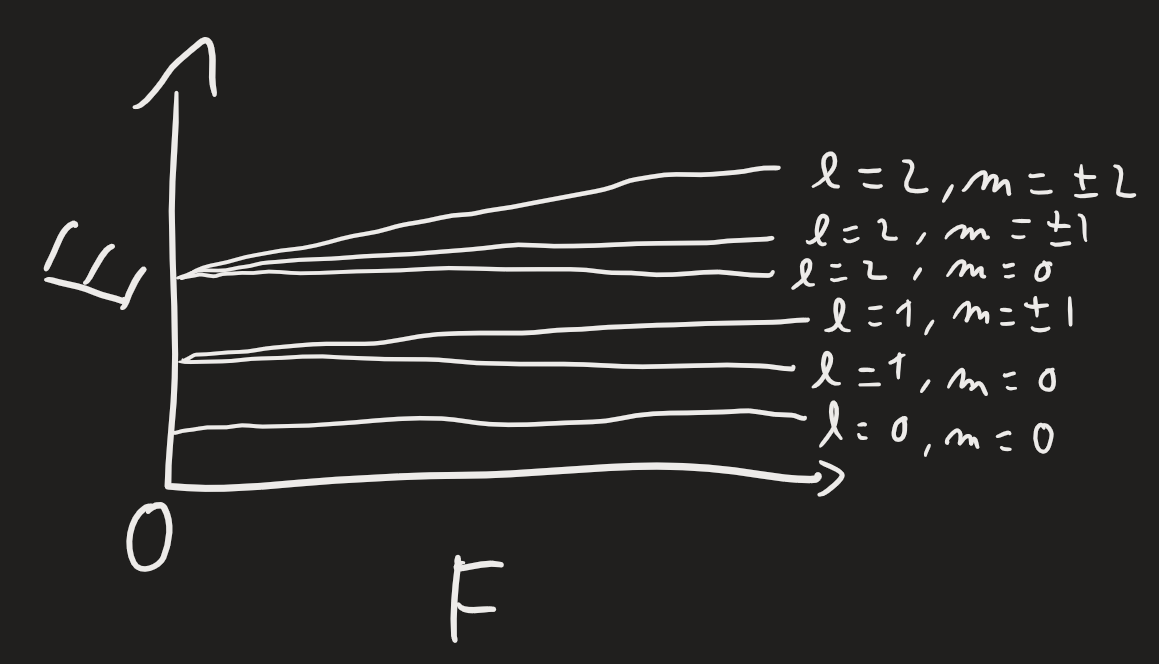
\includegraphics[width = .65\textwidth]{5.8.png}
\caption{Plot of the field and energy as a function of $m$}
\label{fig: 5.8b}
\end{figure}

\subsection*{c)}
The Schrödinger equation is given by:
\[
\left(- \frac{ℏ^2}{2m}∇ + V\right)ψ(r, θ, ϕ) = Eψ(r, θ, ϕ)
\]
Separating the radial out of the function and rewriting the laplacian in spherical coordinates we get:
\[
ψ(r, θ, ϕ) = R(r) Y_{ℓ}^{m} (θ, ϕ)
\]
\[
∇^2 = \frac{1}{r} \frac{∂ }{∂ r} \left(r^2 \frac{∂ }{∂ r}\right) - \frac{1}{ℏ^2r^2}L^2
\]
We can now rewrite the Schrödinger equation with this and the eigenvalues of $L$ as :
\[
- \frac{ℏ^2}{2m} \left(\frac{1}{r} \frac{∂ }{∂ r} \left(r^2 \frac{∂ }{∂ r}\right) - \frac{1}{ℏ^2r^2}l(l+1)\right)R(r) + V(r) R(r) = ER(r)
\]
Redefining $R = u / r$:
\[
\frac{1}{r^2}\frac{∂ }{∂ r} \left(r^2 \frac{∂ }{∂ r} \frac{u}{r}\right) = \frac{1}{r^2} \frac{∂ }{∂ r}\left(r \frac{∂ u}{∂ r} - u\right) = \frac{1}{r} \frac{∂^2 u}{∂ r^2}
\]
Plugging this back in we get:
\[
- \frac{ℏ^2}{2m} \left(\frac{1}{r} \frac{∂^2 u}{∂ r^2} - \frac{l(l+1)}{r^2}\frac{u}{r}\right) + V(r) \frac{u}{r} = E \frac{u}{r}
\]
\[
- \frac{ℏ^2}{2m} \frac{∂^2 u(r)}{∂ r^2} + \frac{ℏ^2l(l+1)}{2mr^2} u(r) + V(r)u(r)=  Eu(r)
\]
This is the form of the1 1D Schrödinger equation with a one-dimensional potential (only $r$ matters). 
\[
V_{1\mathrm{d}} = V(r) + \frac{ℏ^2 l(l+1)}{2mr^2}
\]
The radial wavefunction then becomes:
\[
u(r) = rR(r)
\]

\end{document}